%===============================================================================
% LaTeX sjabloon voor de bachelorproef toegepaste informatica aan HOGENT
% Meer info op https://github.com/HoGentTIN/bachproef-latex-sjabloon
%===============================================================================

\documentclass{bachproef-tin}

\usepackage{hogent-thesis-titlepage} % Titelpagina conform aan HOGENT huisstijl
\usepackage{graphicx}
\usepackage{caption}
\usepackage{refstyle}

%%---------- Documenteigenschappen ---------------------------------------------
% TODO: Vul dit aan met je eigen info:

% De titel van het rapport/bachelorproef
\title{Een Pocket Drone voor schepen}

% Je eigen naam
\author{Daan Verhelst}

% De naam van je promotor (lector van de opleiding)
\promotor{Jens Buysse}

% De naam van je co-promotor. Als je promotor ook je opdrachtgever is en je
% dus ook inhoudelijk begeleidt (en enkel dan!), mag je dit leeg laten.
\copromotor{Pieter Verhelst}

% Indien je bachelorproef in opdracht van/in samenwerking met een bedrijf of
% externe organisatie geschreven is, geef je hier de naam. Zoniet laat je dit
% zoals het is.
\instelling{---}

% Academiejaar
\academiejaar{2019-2020}

% Examenperiode
%  - 1e semester = 1e examenperiode => 1
%  - 2e semester = 2e examenperiode => 2
%  - tweede zit  = 3e examenperiode => 3
\examenperiode{3}

%===============================================================================
% Inhoud document
%===============================================================================

\begin{document}

%---------- Taalselectie -------------------------------------------------------
% Als je je bachelorproef in het Engels schrijft, haal dan onderstaande regel
% uit commentaar. Let op: de tekst op de voorkaft blijft in het Nederlands, en
% dat is ook de bedoeling!

%\selectlanguage{english}

%---------- Titelblad ----------------------------------------------------------
\inserttitlepage

%---------- Samenvatting, voorwoord --------------------------------------------
\usechapterimagefalse
%%=============================================================================
%% Voorwoord
%%=============================================================================

\chapter*{\IfLanguageName{dutch}{Woord vooraf}{Preface}}
\label{ch:voorwoord}

%% TODO:
%% Het voorwoord is het enige deel van de bachelorproef waar je vanuit je
%% eigen standpunt (``ik-vorm'') mag schrijven. Je kan hier bv. motiveren
%% waarom jij het onderwerp wil bespreken.
%% Vergeet ook niet te bedanken wie je geholpen/gesteund/... heeft


%%=============================================================================
%% Samenvatting
%%=============================================================================
% TODO: De "abstract" of samenvatting is een kernachtige (~ 1 blz. voor een
% thesis) synthese van het document.
%
% Deze aspecten moeten zeker aan bod komen:
% - Context: waarom is dit werk belangrijk?
% - Nood: waarom moest dit onderzocht worden?
% - Taak: wat heb je precies gedaan?
% - Object: wat staat in dit document geschreven?
% - Resultaat: wat was het resultaat?
% - Conclusie: wat is/zijn de belangrijkste conclusie(s)?
% - Perspectief: blijven er nog vragen open die in de toekomst nog kunnen
%    onderzocht worden? Wat is een mogelijk vervolg voor jouw onderzoek?
%
% LET OP! Een samenvatting is GEEN voorwoord!
%%---------- Nederlandse samenvatting -----------------------------------------
%
% TODO: Als je je bachelorproef in het Engels schrijft, moet je eerst een
% Nederlandse samenvatting invoegen. Haal daarvoor onderstaande code uit
% commentaar.
% Wie zijn bachelorproef in het Nederlands schrijft, kan dit negeren, de inhoud
% wordt niet in het document ingevoegd.
%\IfLanguageName{english}{%
%\selectlanguage{dutch}
%\chapter*{Samenvatting}
%\lipsum[1-4]
%\selectlanguage{english}
%}{}
%%---------- Samenvatting -----------------------------------------------------
%De samenvatting in de hoofdtaal van het document

\chapter*{\IfLanguageName{dutch}{Samenvatting}{Abstract}}

Jaarlijks sterven er op wereldwijd vlak gemiddeld 320.000 mensen een verdrinkingsdood. Ongeveer 75\% van die 320.000 sterfgevallen komen voort uit overspoeling rampen. Ook vissers hebben een verhoogd risico om te sterven door verdrinking. Daarom is het van cruciaal belang dat er een manier is die ten allen tijde beschikbaar is en helpt bij het zo spoedig mogelijk opsporen van drenkelingen. Een manier zou kunnen zijn dat we een drone op elk schip plaatsen die dan meteen ingezet kan worden voor het zoeken en volgen van de drenkeling alsook het doorsturen van zijn locatie. In deze paper bespreken we de verschillende camera- en dronetechnologieën die beschikbaar zijn om zo de ideale hardware uit te kiezen. Ook zullen we gaan kijken naar de software die nodig is om dit concept te kunnen realiseren. De belangrijkste factoren waarmee rekening gehouden moet worden voor de software wordt ook besproken.
Tenslotte bestuderen we het bestaande systeem waarin we ons concept willen implementeren om zo een zo goed mogelijk plan op te stellen. Daarvoor gaan we kijken naar procedures en wetgevingen die bedrijven en de reddingsdiensten moeten/kunnen volgen. Om dit concept effectief te gaan realiseren zullen er op Europees en/of wereldwijd vlak een aantal wetten of overeenkomsten gerealiseerd moeten worden omtrent het gebruik van drones voor reddingsoperaties. Indien deze wetgevingen en/of overeenkomsten tot stand gebracht kunnen worden, is er niets dat het implementeren van dit concept kan belemmeren. De nodige technologieën zijn beschikbaar en blijven nog steeds evolueren om nog betere prestaties te kunnen leveren. Het is dus zeker mogelijk dat de onderdelen die in deze paper besproken werden, vervangen kunnen worden door betere onderdelen in de toekomst. Extra zaken die we in de toekomst zouden kunnen onderzoeken is de werking van het softwarepakket dat de communicatie tussen het moederschip en de reddingsdiensten zal verzorgen. Ook zouden we in de toekomst onderzoek kunnen doen naar een systeem waarbij schepen, die in de buurt van het incident aanwezig zijn en over een drone beschikken, ook hun drone kunnen inzetten om nog efficiënter tewerk te kunnen gaan.


%---------- Inhoudstafel -------------------------------------------------------
\pagestyle{empty} % Geen hoofding
\tableofcontents  % Voeg de inhoudstafel toe
\cleardoublepage  % Zorg dat volgende hoofstuk op een oneven pagina begint
\pagestyle{fancy} % Zet hoofding opnieuw aan

%---------- Lijst figuren, afkortingen, ... ------------------------------------

% Indien gewenst kan je hier een lijst van figuren/tabellen opgeven. Geef in
% dat geval je figuren/tabellen altijd een korte beschrijving:
%
%  \caption[korte beschrijving]{uitgebreide beschrijving}
%
% De korte beschrijving wordt gebruikt voor deze lijst, de uitgebreide staat bij
% de figuur of tabel zelf.

\listoffigures
%\listoftables

% Als je een lijst van afkortingen of termen wil toevoegen, dan hoort die
% hier thuis. Gebruik bijvoorbeeld de ``glossaries'' package.
% https://www.overleaf.com/learn/latex/Glossaries

%---------- Kern ---------------------------------------------------------------

% De eerste hoofdstukken van een bachelorproef zijn meestal een inleiding op
% het onderwerp, literatuurstudie en verantwoording methodologie.
% Aarzel niet om een meer beschrijvende titel aan deze hoofstukken te geven of
% om bijvoorbeeld de inleiding en/of stand van zaken over meerdere hoofdstukken
% te verspreiden!

%%=============================================================================
%% Inleiding
%%=============================================================================

\chapter{\IfLanguageName{dutch}{Inleiding}{Introduction}}
\label{ch:inleiding}

\section{\IfLanguageName{dutch}{Probleemstelling}{Problem Statement}}
\label{sec:probleemstelling}

Op jaarlijkse basis sterven er gemiddeld 320.000 mensen aan de verdrinkingsdood. Het is echter wel zo dat ongeveer 75\% van deze sterfgevallen, een overspoelingsramp als oorzaak hebben, maar dan nog is het zo dat ongeveer 80.000 mensen buiten een ramp overlijden aan verdrinking. \autocite{WorldHealthOrganisation} Een van de hoofdoorzaken van de verdrinkingsdood is uiteraard het niet op tijd terug vinden van de drenkelingen. Daarom zou het gebruik van een drone een groot verschil kunnen maken. Drones zijn sneller, efficiënter in objectherkenning en kunnen van bovenaf veel meer zien dan de reddingsdiensten zelf. Daarom denken we dat het hebben van een drone op elk schip een goede oplossing kan zijn om mensen sneller op te sporen en zo het aantal sterfgevallen door verdrinking nog meer te drukken.

\section{\IfLanguageName{dutch}{Onderzoeksvraag}{Research question}}
\label{sec:onderzoeksvraag}

Welke hardware is het beste om te gebruiken bij reddingsacties op zee?

\begin{itemize}
	\item Welke camera's dient men te gebruiken?
	\item Welke drone(s) dient men te gebruiken?
\end{itemize}

Welke software is het beste voor het herkennen van mensen op zee?

\begin{itemize}
	\item Is een automatisch pilootsysteem voldoende? Moeten we combineren met handmatige besturing?
	\item Welk objectherkenningsalgorithme is het beste voor objectherkenning op zee?
\end{itemize}

Wat is de beste manier om drones te implementeren in de bestaande situatie van de zeevaartsector?

\section{\IfLanguageName{dutch}{Onderzoeksdoelstelling}{Research objective}}
\label{sec:onderzoeksdoelstelling}

Op het einde van deze bachelorproef moeten we in staat zijn om een aanbeveling te doen voor zowel de hardware als de software (dit aan de hand van metingen) die gebruikt kunnen worden voor het inzetten van drones bij reddingsacties. Ook moeten we concreet kunnen aantonen hoe de drones binnen het huidige systeem van de zeevaartsector kan verwerkt worden.

\section{\IfLanguageName{dutch}{Opzet van deze bachelorproef}{Structure of this bachelor thesis}}
\label{sec:opzet-bachelorproef}

% Het is gebruikelijk aan het einde van de inleiding een overzicht te
% geven van de opbouw van de rest van de tekst. Deze sectie bevat al een aanzet
% die je kan aanvullen/aanpassen in functie van je eigen tekst.

De rest van deze bachelorproef is als volgt opgebouwd:

In Hoofdstuk~\ref{ch:stand-van-zaken} wordt een overzicht gegeven van de stand van zaken binnen het onderzoeksdomein, op basis van een literatuurstudie.

In Hoofdstuk~\ref{ch:methodologie} wordt de methodologie toegelicht en worden de gebruikte onderzoekstechnieken besproken om een antwoord te kunnen formuleren op de onderzoeksvragen.

% TODO: Vul hier aan voor je eigen hoofstukken, één of twee zinnen per hoofdstuk

In Hoofdstuk~\ref{ch:conclusie}, tenslotte, wordt de conclusie gegeven en een antwoord geformuleerd op de onderzoeksvragen. Daarbij wordt ook een aanzet gegeven voor toekomstig onderzoek binnen dit domein.
\chapter{\IfLanguageName{dutch}{Stand van zaken}{State of the art}}
\label{ch:stand-van-zaken}

% Tip: Begin elk hoofdstuk met een paragraaf inleiding die beschrijft hoe
% dit hoofdstuk past binnen het geheel van de bachelorproef. Geef in het
% bijzonder aan wat de link is met het vorige en volgende hoofdstuk.

% Pas na deze inleidende paragraaf komt de eerste sectiehoofding.

\section{Hardware}

\paragraph{Inleiding}
In dit deel van de paper zullen we de noodzakelijke en optionele hardware bespreken die gebruikt kunnen/moeten worden voor het optimaliseren van de efficiëntie van drones bij het detecteren van drenkelingen op diepzee. We nemen even de tijd om de verschillende beschikbare types van camera's te bestuderen. We zullen proberen om de meest geschikte camera te vinden voor het assisteren bij reddingsoperaties. Bij het vinden van deze optimale camera moet uiteraard rekening gehouden worden met verscheidene factoren zoals kledij, snelheid van herkenning van drenkelingen, etc. Ook zullen we een vergelijking maken tussen verschillende drones die momenteel beschikbaar zijn. Factoren zoals snelheid, stabiliteit, robuustheid, kostprijs, etc zullen hier van groot belang zijn. We zullen ook de voor en nadelen van zowel één als meerdere drones inzetten bespreken. Ten slotte bespreken we nog enkele optionele onderdelen die eventueel ook gebruikt kunnen worden voor het optimaliseren van de overlevingskans van de drenkeling. Hier denken we aan een mogelijkheid tot communicatie tussen boot en drenkeling, het brengen van een reddingsboei, etc.

\subsection{Optimale optische technologie voor het detecteren van drenkelingen}

\paragraph{Normale camera}

\subitem
De normale camera, die we gebruiken voor het maken van mooie foto's, is ons allemaal bekend. Elke smartphone heeft tegenwoordig camera's die prachtige en gedetailleerde foto's kan maken en de ontwikkeling van deze technologie is nog steeds lopende. Maar wat is zo'n camera nu eigenlijk? Hoe werkt het en hoe kunnen wij het gaan gebruiken voor de uitwerking van ons idee? (nl. het gebruik van camera's voor persoondetectie)

\subitem
Wat is een camera? Een camera is een toestel dat in staat is om een beeld die zich voor de lens bevindt vast te leggen. Eens de persoon, die de foto wil trekken, op de knop drukt om het beeld vast te leggen, opent een shutter die tot dan het licht tegenhield. De lens zal dan het binnenkomende licht op focussen zodat het op een fotografische film of digitale sensor terecht komt. Aan de hand van deze photografische film of digitale sensor, kan dan een digitale representatie van de getrokken personen, het getrokken object of landschap. Als men nu dit proces meerdermalen herhaald en alle foto's die getrokken werden op een snel tempo na elkaar tonen, dan krijg je een videofragment in plaats van een enkele foto. Om dit te kunnen doen moet men natuurlijk aan een zeer hoog tempo foto's kunnen trekken zodat verandering in de getrokken omgeving, geleidelijk aan weergegeven worden en niet in sprongen. De snelheid waarmee de foto's genomen worden, wordt uitgedrukt in frames per seconde waarbij een frame een synoniem is voor een foto. Een veel voorkomend frame-rate bij videocamera's is 24 frames per seconde wat dus wil zeggen dat er per seconde 24 foto's genomen worden. Om deze nu aan een correcte snelheid af te spelen moeten de afbeeldingen ook aan een snelheid van 24 frames per seconde weergegeven worden. De resolutie van een foto is ook een belangrijke factor bij fotografie. Dit wordt uitgedrukt in pixels en hangt af van het aantal fotodiodes op de digitale sensor. Deze fotodiodes zijn de componenten die de lichtinval opvangen en omzetten naar digitale data van de foto. Een pixel is een, meestal heel klein, stukje van de afbeelding die een bepaalde kleur aanneemt. \autocite{DigitalCameras}

\subitem
Hoe kunnen wij zo'n camera nu gaan toepassen op de detectie van drenkelingen op diepzee? Zoals eerder vermeld werd, kunnen we aan een heel hoog tempo foto's nemen aan een bepaalde resolutie om zo een videofragment vast te leggen. Indien we nu elk van deze frames zouden laten analyseren door een algoritme, die in staat is om mensen te herkennen, zouden we op die manier aan persoonherkenning kunnen doen. Een probleem met deze camera is dat het sterk afhankelijk is van voldoende lichtinval. In zeer donkere omstandigheden zoals de nacht op zee, zou dit geen goede oplossing zijn. 

\paragraph{IR-Camera}

\subitem
Zoals we in de vorige paragraaf besproken hadden, is het zo dat normale camera's, in donkere omstandigheden, niet voldoende zouden zijn voor het detecteren van drenkelingen op zee. Er zou niet voldoende lichtinval zijn om duidelijke afbeeldingen te maken waaruit een algoritme dan een mens kan herkennen. Daarom zijn er andere technologieën die op een zeer gelijkaardige manier beelden kunnen vastleggen maar toch een ander resultaat verkrijgen. Een van deze alternatieve technologieën is infra-rood camera's. 

\subitem
Wat is nu het verschil tussen een gewone camera en een infra-rood camera? Zoals eerder vermeld is het eigenlijk een zeer klein verschil tussen de twee camera's. Het werkt ook met een lens, een shutter en sensoren. Het verschil is dat, bij een infra-rood camera, een infra-rood sensor array gebruikt wordt. Deze sensoren zijn in staat om infra-rood energie te detecteren en deze informatie om te zetten naar een afbeelding. Het menselijk lichaam geeft veel verschillende stralingen af maar infra-rood licht is een van de meest aanwezige vormen van straling.

\subitem
Om deze technologie nu te gaan toepassen op het detecteren van drenkelingen op zee, kunnen we zeer gelijkaardig te werk gaan. Een infra-rood camera kan namelijk, op een gelijkaardige manier aan de normale camera, heel snel fotos nemen. Op die manier kunnen we videomateriaal maken door ze opnieuw op eenzelfde frequentie af te spelen. Ook kunnen we frame per frame gaan analyseren om na te gaan of een drenkeling op dat frame te zien is. Het voordeel aan infrarood camera's is dat, het menselijk lichaam die veer infra-roodstralingen uitstraalt, sterk oplicht op een frame of foto die genomen werd door een infra-rood camera. Hierdoor is een infra-rood camera een zeer goede optische technologie in donkere omgevingen. 

\paragraph{Warmtecamera}

\subitem
Zoals vermeld in de bovenstaande paragraaf, zijn er betere alternatieven voor een gewone camera. De warmtecamera is hier nog een voorbeeld van. Deze camera is ook weer heel gelijkaardig aan de gewone camera met opnieuw als grootste verschil, de soort straling die gedetecteerd wordt. Bij warmtecameras wordt er ook licht uit het infra-rode spectrum opgevangen maar deze keer in het lange infra-rood bereik waar men bij infra-rood camera's eerder het licht uit de near-infra-rode regio gaat opvangen. Het licht binnen de near-infra-rode regio is net niet zichtbaar is met het blote oog. Het grote nadeel van infra-rood camera's is dat er een minimum hoeveelheid licht moet zijn vooraleer het kan werken. Dit is waar warmtecamera's beter zijn dan infra-rood camera's. Omdat warmtecamera's gebruik maken van licht uit het lange infra-rood bereik, zijn deze camera's niet afhankelijk van ander licht. Deze camera registreert enkel de warmte die een mensenlichaam uitstraalt. Daarom is dit een superieure optie ten opzichte van de andere camera's. Deze kan zowel 's nachts als overdag gebruikt worden. 

\subitem
Deze camera kunnen we dus op een gelijkaardige manier in gebruik nemen. We laten foto's of frames nemen die we dan zullen analyseren aan de hand van een algoritme. Op basis daarvan kunnen we dan bepalen of er een drenkeling in beeld is of niet. 



\subsection{Optimale drone voor reddingsacties op zee}

\subitem
Er zijn verschillende zaken die in rekening gebracht moeten worden wanneer we een drone moeten kiezen. Zo moeten we bijvoorbeeld kijken naar de materialen die gebruikt werden bij de productie van de drone, de mate waarin het geprogrammeerd kan worden om autonoom op pad te gaan, de kostprijs en beschikbaarheid van de drone en de bijbehorende vervangstukken, de reikwijdte van het toestel, de hefkracht van het toestel en de hoelang de drone vliegende kan blijven zonder opgeladen te moeten worden. Eerst zullen we een goedkopere consumer-grade drone bespreken. We kijken of het voordeliger is om goedkope toestellen te gebruiken en ze simpelweg te vervangen bij schade of dat we een duurdere industrial-grade drone nemen met vervangstukken.

\paragraph{Consumer-grade drone}

\subitem
Het eerste toestel dat we gaan bekijken is een drone van bedrijf Ryze Robotics. \autocite{CheapDrone} Het kost iets minder dan 110 euro wanneer we het aankopen via het officiële verkooppunt \autocite{CheapDroneOfficial}. 

We weten niet uit welk materiaal deze drone opgebouwd is wat wil zeggen dat we dus ook niet weten hoe resistent deze drone is tegen heftigere omstandigheden. Het is niet programmeerbaar wat wil zeggen dat we iemand de drone moeten laten besturen en iemand de live beelden moeten laten analyseren. Dit wil dus zeggen dat we 2 mensen nodig hebben per drone. Er is geen mogelijkheid om een reddingsband naar de drenkeling te vervoeren door een gebrek aan opties voor een robotische arm. Ook herstelling van een drone is niet mogelijk door het gebrek aan vervangstukken. Bij schade moeten we een nieuwe drone aanschaffen. De reikwijdte van de drone is slechts 100 meter. Indien de drenkeling pas na een paar minuten vermist wordt, is het mogelijk dat de drone niet ver genoeg kan vliegen om de drenkeling te detecteren. De vliegtijd is slechts 13 minuten dus indien de drenkeling niet binnen 13 minuten terug gevonden en gered wordt, verliest de drone zijn waarde.
De drone moet namelijk in staat zijn om zijn locatie te versturen naar de reddingstroepen. De snelheid van 8 meter / seconde zou wel voldoen.
Over het algemeen kunnen we stellen dat deze drone niet geschikt is voor onze toepassing.

\paragraph{Industrial-grade drone}

\subitem
Nu gaan we kijken naar een voorbeeld van een industrial-grade drone die bedoeld is voor gebruik in bedrijven en organisaties. Deze drone is heel wat duurder dan een consumer-grade drone maar zou heel wat voordelen hebben.

Deze drone is bijvoorbeeld geconstrueerd uit materialen die corosieresistent zijn zodat het in verscheidene weersomstandigheden kan vliegen, de drone kan automatisch geactiveerd worden, alsook geprogrammeerd worden om een bepaald patroon te volgen, de optie voor een robotische arm is er, indien de batterij plat is, kan deze vervangen worden zodat de drone meteen terug op pad kan. Ook heeft het een zeer accurate locatie-apparatuur waardoor het zeer duidelijk de locatie van de drenkeling kan doorsturen.Het heeft ook een parachute voor bij noodlandingen. Dit kan helpen om schade te beperken en dus ook kosten aan de drone. Live beelden zijn mogelijk. Tenslotte is er ook nog de kist die er speciaal voor werd ontworpen. In deze kist, zit de drone veilig en wordt het opgeladen indien nodig. 

Dit is duidelijk een betere optie voor deze toepassing.

\paragraph{Een versus meerdere drones}

\subitem
Het snel vinden van drenkelingen op zee is cruciaal voor de overlevingskansen van de drenkeling. Dit roept de volgende vraag op. Is één drone voldoende of hebben we er meer nodig? Om dit te bepalen moeten we bepalen hoeveel oppervlakte één drone kan onderzoeken binnen een bepaalde tijdseenheid. Neem nu dat de drone een hoogte van 120 meter aanhoudt en dat de drone een oppervlakte van 1600 vierkante meter "ziet". Combineer dit nu met het feit dat de hierboven besproken drone een snelheid van 10m/s kan aanhouden. Hieruit kunnen we afleiden dat de drone, iedere 4 seconden, 1600 vierkante meter kan inspecteren met als gevolg dat we in 1 minuut, 24 vierkante kilometer aan oppervlakte kunnen doorzoeken. Het is duidelijk dat één drone voldoende zal zijn voor het vinden van drenkelingen. 

\subsection{Extra opties}

\subitem
De drone zelf op zich is reeds een grote aanwinst bij reddingsoperaties maar het kan nog beter. Door de drone uit te rusten met een aantal extra opties, kunnen we de efficiëntie van een drone bij reddingsoperaties nog verbeteren. Daarom zullen we in deze subsectie een aantal ideeën bespreken voor optionele extenties voor de drone.  

\paragraph{Luidsprekers en een microfoon voor communicatie}

\subitem
Stel iemand valt overboord in het water. De drone wordt geactiveerd en vindt na een bepaalde tijd de drenkeling terug. Wat doet de drone terwijl de reddingsbrigade onderweg is? Een idee is om een luidspreker en microfoon in de drone te verwerken om communicatie op afstand mogelijk te maken. Zo kunnen we misschien de kalmte van de drenkeling bewaren. Ook zouden we kalmerende muziek kunnen afspelen om opnieuw de kalmte te bewaren. 
De microfoon kan ook dienen als een geluidsdetector. Als de drenkeling luid roept naar de drone die hij/zij ziet passeren, dan zou dit ook als middel voor localisatie kunnen dienen.

\paragraph{Vuurfakkel voor signalisatie}

Nog een optie zou kunnen zijn dat we aan de hand van een klauw een vuurfakkel naar de drenkeling brengen zodat de reddingsoperatoren sneller zien waar de is. Dit zou tijd uitsparen in donkere omstandigheden. Hoewel de warmtecamera dan de exacte locatie uit het oog zal verliezen, door de grote hoeveelheid hitte die de vuurfakkel uitstoot, kan een schatting van de locatie nog steeds behouden worden en voor de exacte locatie dient uiteraard de vuurfakkel. 

\section{Software}

\paragraph{Inleiding}
In vorige sectie hebben we de noodzakelijke en optionele hardware, zoals drones en camera's, besproken. Uiteraard is hardware op zichzelf niet voldoende. Deze hardware moet door een of andere software bestuurd en ondersteund worden en dat is precies wat we in deze sectie gaan bespreken. We zullen onderzoek doen naar het al dan niet handmatig of ge-automatiseerd besturen van de drone. Een combinatie is uiteraard ook een optie. Daarna zullen de voordelen en nadelen van verscheidene herkenningsalgorithmen gaan vastleggen om zo de meest optimale algorithmen eruit te kunnen kiezen.

\subsection{Besturing van de drone}

\paragraph{Handmatig}

\subitem
Het handmatig besturen van de drone heeft zijn voor- en nadelen. De voordelen zijn dat je meer controle hebt over de drone waardoor je gerichter kan werken. Als je weet waar de drenkeling ongeveer zou kunnen zijn zou je de drone zelf in die richting kunnen besturen om zo sneller de drenkeling te vinden. De nadelen zijn dat mensen niet even accuraat tewerk kunnen gaan als we het vergelijken met een computer. Nog een nadeel van het handmatig besturen van de drone is dat men mensen zal moeten opleiden voor het besturen van die drone. 

\paragraph{Automatisch}

\subitem
De drone laten besturen door een computer systeem heeft ook zijn voor- en nadelen. De voordelen zijn dat de computer, op basis van coördinaten, een veel accurater grid-patroon kan volgen en dus minder fouten maakt. Door de rekenkracht van de computer kan de drone ook maximaal benut worden. Het grote nadeel hieraan is dat een computer systeem niet over zoiets als een intuïtie beschikt. Het zal zijn voorgeprogrammeerd pad afleggen en niets meer of minder dan dat.  

\paragraph{Combinatie}

\subitem
Gezien beide zowel voor als nadelen heeft is het misschien beter van beide opties te combineren om zo zoveel voordelen als mogelijk is te behouden. We zouden bijvoorbeeld handmatig kunnen zoeken in de algemene richting waar men vermoed de drenkeling terug te vinden. Na het vinden van de drenkeling kan de computer dan overnemen voor het volgen van de drenkeling tot de drenkeling uiteindelijk gered wordt. 

\subsection{Herkenningssoftware}

\paragraph{Voordelen}

\lipsum[1-2]

\paragraph{Nadelen}

\lipsum[1-2]

\section{Implementatie}

\paragraph{Inleiding}

\subitem
Nu dat we voldoende voorkennis hebben omtrent zowel hardware als software alsook de meest efficiënte hardware en software bepaald hebben voor deze toepassing (nl. reddingsacties op diepzee) kunnen we verder gaan naar de implementatiefase van dit concept. Voordat we een goed voorstel kunnen geven voor de implementatie van drones bij reddingsacties moeten we uiteraard een goed beeld hebben van de huidige situatie binnen de zeevaartsector. Daarom zullen we ons in deze sectie eerst gaan verdiepen in de bestaande procedures die bedrijven en reddingsdiensten moeten volgen, alsook de wetten rond het gebruik van drones. Daarna zullen we, met alle vooraf vergaarde kennis, de effectieve acties en implementatie van de drone gaan vastleggen. We bespreken dan alle stappen van opstijgen en landen tot het vastleggen van acties die de drone zou ondernemen in het geval van het detecteren van een drenkeling. 

\subsection{Bestaande procedures en verwerking}

\paragraph{Wetten rond dronegebruik}

\lipsum[1-2]

\paragraph{Procedures van Reddingsdiensten}

\lipsum[1-2]

\paragraph{Procedures van bedrijven in de scheepvaartsector}

\lipsum[1-2]

\paragraph{Verwerking van drones in bestaand systeem}

\lipsum[1-2]

\subsection{Opstijgen en landen op zee}

\paragraph{Vertrek}

\lipsum[1-2]

\paragraph{Recovery}

\lipsum[1-2]

\subsection{Acties bij detectie van een drenkeling}

\subitem
Wat moet de drone nu doen wanneer het de locatie van de drenkeling ontdekt heeft. Er zijn verscheidene zaken die de drone kan en/of moet doen. De drone moet aangeven dat het iets of iemand gedetecteerd heeft. Er kan geopteerd worden voor het landen van de drone om de batterij van de drone te sparen tot de reddingsdiensten arriveren of de drone kan in de lucht blijven. Tot slot kan de drone gebruikt worden om de kalmte van de drenkeling te bewaren zodat hij of zij niet te veel energie verdoet en het zo langer kan uithouden tot de reddingsdiensten aankomen. Deze zaken zullen we nu bespreken.

\paragraph{Signalisatie van locatie}

\subitem
De locatie van de drone is hoe dan ook bekend door de localisatie die in de drone ingebouwd is. Hoe kunnen we dan weten wanneer de drone iets ontdekt heeft? Eerst en vooral zou de drone tot stilstand komen wat zichtbaar zou zijn op de live feed van de drone. Dat zou één methode kunnen zijn voor het bepalen van de locatie van de drenkeling. Dit is natuurlijk niet de beste oplossing die we met deze technologie kunnen bereiken. We zouden er bijvoorbeeld ook voor kunnen zorgen dat de drone zelf een signaal uitzendt naar het computersysteem op het schip zelf. Zo kunnen de reddingsdiensten meteen naar de locatie van het signaal navigeren met een hoge waarschijnlijkheid, de drenkeling terug te vinden.  

\paragraph{Landen versus vliegen}

\subitem
Eens de drone de locatie van de drenkeling ontdekt heeft en het signaal gegeven heeft zodat de reddingsdiensten ook op de hoogte gebracht zijn, kan de drone 2 zaken doen: landen op zee of in de lucht blijven. Beide opties hebben voordelen en nadelen die in rekening gebracht moeten worden. In de lucht blijven heeft als voordeel dat het veel gemakkelijker is om de drenkeling te blijven volgen om zo een accurate locatie door te kunnen blijven geven. Een groot nadeel is dat het veel meer batterij zou verbruiken en als de reddingsdiensten niet op tijd aankomen zou het rampzalig zijn als de drone vroegtijdig zou moeten terug keren. Ook moeten we rekening houden met het feit dat reddingsacties dikwijls ondernomen worden aan de hand van een reddingshelicopter. Dit wil zeggen dat er een systeem ontwikkeld en geïmplementeerd zal moeten worden zodat de drone weet wanneer het uit de weg moet gaan voor de helicopter. De drone in de lucht houden heeft dus duidelijk heel wat nadelen. Wanneer we de drone op het water laten landen, dan moeten de rotoren van de drone niet actief zijn. Dit is positief voor de batterijduur van de drone. Als alle stroom gebruikt kan worden voor signalisatie, dan is er veel minder risico dat de drone moet terugkeren vooraleer de drenkeling gered werd door reddingsdiensten. Een nadeel is echter wel dat het voor de drone veel moeilijker is om de drenkeling in de gaten te houden. Er moet ook gezorgd worden dat de drone geen obstakel vormt voor de reddingsactie indien men boten gebruikt. Een goede oplossing zou kunnen zijn dat de drone uitgerust is met een airbagachtig systeem zodat het een reddingsboei kan vormen. De drone kan op een veilige afstand landen en de drenkeling kan er dan naartoe zwemmen. Dit maakt het ook gemakkelijker om via een microfoon te communiceren met mensen op het schip. 

\paragraph{Kalmte van de drenkeling bewaren}

Paniek is iets heel gevaarlijk in elke mogelijke situatie die je kan bedenken. Het is al vaak gebleken dat mensen, die in paniek slaan, het vermogen om rationeel te reageren verliezen. Dit feit leidt dikwijls tot ongelukkige en soms zelfs dodelijke ongevallen. Op zee kan paniek echter andere gevolgen teweeg brengen. Indien een drenkeling paniek begint te vertonen, zal hij of zij meer energie gaan verbruiken door hyperventilatie, overbodige bewegingen en eventueel door huilen of roepen om hulp. Al deze extra energie verbruiken kan gevaarlijk zijn omdat de 

\chapter{Implementatie}
\label{ch:implementatie}

\paragraph{Inleiding}

Nu dat we voldoende voorkennis hebben omtrent zowel hardware als software alsook de meest efficiënte hardware en software bepaald hebben voor deze toepassing (nl. reddingsacties op diepzee) kunnen we verder gaan naar de implementatiefase van dit concept. Voordat we een goed voorstel kunnen geven voor de implementatie van drones bij reddingsacties moeten we uiteraard een goed beeld hebben van de huidige situatie binnen de zeevaartsector. Daarom zullen we ons in dit onderdeel gaan verdiepen in de bestaande procedures die bedrijven en reddingsdiensten moeten volgen alsook de wetten rond het gebruik van drones op zee. Daarna zullen we, met alle vooraf vergaarde kennis, de effectieve acties en implementatie van de drone gaan vastleggen. We bespreken dan alle stappen van opstijgen en landen tot het vastleggen van acties die de drone zou ondernemen in het geval van het detecteren van een drenkeling. 

\section{Bestaande procedures, wetten en verwerking}

\paragraph{Wetten rond dronegebruik op zee}

Op dit moment is het bijzonder moeilijk om dit concept in België te gaan implementeren. Door de KB RPAS wet (sinds 2016) zijn de enige instanties die onmiddellijk een drone mogen inzetten indien zij het nodig achten de politie, de brandweer en de civiele bescherming van België. Alle andere instanties zijn verplicht om heel wat papieren in te vullen en een aanvraag in te dienen. Op 1 januari 2021 zal er echter een wetgeving doorgevoerd worden op Europees niveau waardoor, indien er een gecertificeerde piloot aanwezig is, een drone ingezet mag worden zonder al dat papierwerk in te moeten vullen. Dan kunnen we dit concept wel implementeren, althans in België. 

Alle oceanen en zeeën zijn opgedeeld in SRRs of Search and Rescue Regions. Voor België is dit de Maritieme Search and Rescue Region (MSRR). Ook is het luchtruim opgedeeld in FIRs of Flight Information Regions. Voor het implementeren van dit concept moeten we beide zones dus in rekening brengen. Dit wil dus ook zeggen dat de drone enkel ingezet kan worden indien ze zich in wateren bevinden die dit, volgens de wetgeving van het respectievelijke land, toestaan. Voor het implementeren van dit concept zal dus een Europese of wereldwijde overeenkomst tot stand gebracht moeten worden met meerdere landen die ook interesse hebben in dit concept.   

\paragraph{Procedures van Reddingsdiensten}

Eens de reddingsdiensten een oproep binnenkrijgen in verband met een drenkeling en voldoende informatie vergaard hebben zullen zij vertrekken naar de plaats van het incident. Eens de reddingsdiensten daar aangekomen zijn zullen zij, indien het slachtoffer nog niet gevonden is, een zoekactie uitvoeren met behulp van boten en/of helikopters en aan de hand van een drift- of zoekplan. Ook staan zij in voor het coördineren en synchroniseren van andere reddingseenheden die eventueel ook ingezet werden. Eens de drenkeling gevonden is en vervolgens in veiligheid gebracht is, moeten de reddingsdiensten deze informatie doorgeven aan de juiste instantie. Voor België is dit bijvoorbeeld het Maritieme Reddings- en Coördinatiecentrum (MRCC). 

\paragraph{Procedures van bedrijven in de scheepvaartsector}

Bij een man-over-boord incident mag het personeel van het vaartuig zelf onmiddellijk actie ondernemen. Zij moeten niet wachten op de reddingsdiensten om zelf een poging te wagen, de drenkeling te redden. Het kan wel zijn dat de SAR mission coördinatoren (SAR staat voor Search And Rescue), de poging van het moederschip stop zet indien het verderzetten ervan inefficiënt geacht wordt.

\paragraph{Verwerking van drones in het bestaande systeem}

De eerste stap van de implementatie van dit concept zal inhouden dat, op Europees of wereldwijd vlak, zoveel mogelijk landen een overeenkomst verwezelijken dat dit concept toelaat. Indien een Belgisch schip zich in Spaanse wateren begeeft, dan moet Spanje het inzetten van de drone toelaten zonder dat er om gevraagd moet worden om zo snel mogelijk de drenkeling te vinden en te volgen. Anders verliest de drone opnieuw zijn waarde.
Eens dit gerealiseerd is, moeten we een gemeenschappelijk netwerk opstellen dat alle betrokken partijen in staat stelt om vlot met elkaar te communiceren. Eens de drone opstijgt, moet een signaal automatisch gegeven worden aan de reddingsdienst in kwestie, waarna deze dienst meteen contact kan opnemen met het moederschip waartoe de drone behoort, om verder te kunnen communiceren. Eens de reddingsdiensten bijna op de plaats van het incident aangekomen zijn, kan de gecertifieerde piloot, de drone ver genoeg verwijderen van de drenkeling zodat het niet in de weg van de reddingsdiensten vliegt. Dit kan ook verwerkt worden in de software van de drone zodat deze zich automatisch op een veilige afstand plaatst. Indien de drenkeling nog niet gevonden werd, kunnen de reddingsdiensten advies geven in verband met zoekpatronen die de crew kan volgen of vragen de drone terug te trekken zodat zij zelf de zoektocht kunnen verderzetten.

\section{Opstijgen en landen op zee}

In normale omstandigheden zou het landen en opstijgen met een drone geen overdreven moeilijke onderneming mogen zijn. Je plaatst de drone op een vlak oppervlak en de drone kan verticaal opstijgen. Gelijkaardig voor het landen kan je simpelweg de drone naar de landingsbaan of het landingsplatform sturen en dan de hoogte van de drone geleidelijk aan verlagen. Opstijgen en landen op een schip is echter niet zo gemakkelijk. Terwijl je op land een stilstaand platform hebt, is een schip constant in beweging. We willen uiteraard niet dat de drone tegen het schip of het materiaal op het schip botst. 

\paragraph{Vertrek}

Voor het vertrek moeten we dus rekening houden met de snelheid van het schip alsook de koers die het schip volgt want als we verticaal zouden opstijgen, is het niet onmogelijk dat de nog steeds varende boot, de stationaire drone onderschept. Hoewel het schip waarschijnlijk wel gestopt zal worden bij een man-over-boord incident, staat een groot schip niet meteen stil. We willen echter wel zo snel mogelijk de drone inzetten zodat de drenkeling zo snel mogelijk gevonden en gevolgd kan worden. Daarom moet de drone ergens kunnen opstijgen waar het geen obstakels kan tegenkomen waartegen het zou kunnen vliegen. Voorbeelden hiervan zijn aan de rand van het schip, op een verhoogd punt zoals een balkon of helemaal achteraan het schip. Deze locaties zijn uiteraard verschillend voor elk schip aangezien schepen veel verschillende vormen aan kunnen nemen.

\paragraph{Recovery}

Eens de drone zijn opdracht voltooid heeft, kunnen we de drone uiteraard niet gewoon achterlaten. We willen deze terug zien te krijgen zodat het bij het volgende incident opnieuw gebruikt kan worden. We kunnen enerzijds een "return to home" zender implementeren zodat de drone ten allen tijde weet waar het terecht kan na de reddingsactie of een gecertifieerd piloot kan het manueel terug vliegen. Deze zender geeft zijn locatie door aan de drone zodat de drone steeds de weg naar het schip terug kan vinden. We zitten echter wel opnieuw met het probleem dat een schip nooit volledig stil staat. Dit kan landen moeilijker maken, zeker als het schip nog aan vaarsnelheid voortbeweegt maar dit is vrij onwaarschijnlijk. Een minimum aan beweging van het schip is cruciaal.

\section{Acties bij detectie van een drenkeling}

Wat moet de drone nu doen wanneer het de locatie van de drenkeling ontdekt heeft. Er zijn verscheidene zaken die de drone kan en/of moet doen. De drone moet aangeven dat het iets of iemand gedetecteerd heeft. Er kan geopteerd worden voor het landen van de drone, met opblaasbare voetstukken, om de batterij van de drone te sparen tot de reddingsdiensten arriveren of de drone kan in de lucht blijven. Tot slot kan de drone gebruikt worden om de kalmte van de drenkeling te bewaren zodat hij of zij niet te veel energie verdoet en het zo langer kan uithouden tot de reddingsdiensten aankomen. Deze zaken zullen we nu bespreken.

\paragraph{Signalisatie van locatie}

Het is belangrijk dat, wanneer de drenkeling gevonden is, de drone zijn locatie doorgeeft aan zowel de crew van het schip als de reddingsdiensten. De crew van het schip zal ook al kunnen zien op de monitor wanneer de drone stil komt te staan. Dat zou één methode kunnen zijn voor het bepalen van de locatie van de drenkeling maar dit is natuurlijk niet de beste oplossing die we met deze technologie kunnen bereiken. Het automatisch signaleren en locatie delen zou een veel effectievere oplossing zijn. Zo kunnen de reddingsdiensten meteen naar de locatie van het signaal navigeren met een hoge waarschijnlijkheid, de drenkeling daar terug te vinden.  

\paragraph{Landen versus vliegen}

Eens de drone de locatie van de drenkeling ontdekt heeft en het signaal gegeven heeft zodat de reddingsdiensten ook op de hoogte gebracht zijn, kan de drone 2 zaken doen: landen op zee of in de lucht blijven. Beide opties hebben voordelen en nadelen die in rekening gebracht moeten worden. In de lucht blijven heeft als voordeel dat het veel gemakkelijker is om de drenkeling te blijven volgen om zo een accurate locatie door te kunnen blijven geven. Een groot nadeel is dat het  meer batterij zal verbruiken en als de reddingsdiensten niet op tijd aankomen zou het rampzalig zijn als de drone vroegtijdig zou moeten terug keren. Ook moeten we rekening houden met het feit dat reddingsacties dikwijls ondernomen worden aan de hand van een helikopter. Dit wil zeggen dat er een systeem ontwikkeld en geïmplementeerd zal moeten worden zodat de drone weet wanneer het uit de weg moet gaan voor de helikopter of dat een gecertifieerd piloot de drone uit de weg navigeert. De drone in de lucht houden heeft dus duidelijk heel wat nadelen. Als alle stroom gebruikt kan worden voor signalisatie, dan is er veel minder risico dat de drone moet terugkeren vooraleer de drenkeling gered werd door reddingsdiensten. Een nadeel is echter wel dat het voor de drone veel moeilijker is om de drenkeling in de gaten te houden. Er moet ook gezorgd worden dat de drone geen obstakel vormt voor de reddingsactie indien men boten gebruikt. Een goede oplossing zou kunnen zijn dat de drone uitgerust is met een airbagachtig systeem zodat het een reddingsboei kan vormen. De drone kan op een veilige afstand landen en de drenkeling kan er dan naartoe zwemmen. Dit maakt het ook gemakkelijker om via een microfoon te communiceren met mensen op het schip. 

\paragraph{Kalmte van de drenkeling bewaren}

Paniek is iets heel gevaarlijk in elke mogelijke situatie die je kan bedenken. Het is al vaak gebleken dat mensen, die in paniek slaan, het vermogen om rationeel na te denken verliezen. Dit feit leidt dikwijls tot ongelukkige en soms zelfs dodelijke ongevallen. Op zee kan paniek echter nog andere gevolgen teweeg brengen. Indien een drenkeling in paniek begint te slaan, zal hij of zij meer energie gaan verbruiken door hyperventilatie, overbodige bewegingen en eventueel door huilen of roepen om hulp. We moeten ervoor zorgen dat de drenkeling deze extra energie spaart zodat hij of zij niet bezwijkt door vermoeidheid.
\chapter{Proof of concept}
\label{ch:proofofconcept}

\section{Inleiding}

Nu we een duidelijker beeld hebben van de hard- en software die op dit moment op de markt beschikbaar is alsook hoe we dit concept zouden kunnen implementeren, kunnen we dit deels uitwerken in de vorm van een scenario.
Het scenario begint op het moment waar een bemanningslid (of klant in het geval van cruiseschepen) overboord gevallen is. De eerste reactie van het bevoegd personeel is om de drone uit te halen en volledig voor te bereiden voor vertrek alsook de reddingsdiensten te contacteren en over het incident in te lichten. Op die manier kunnen de reddingsdiensten zo snel mogelijk vertrekken.
Na het inlichten van de reddingsdiensten begint onze test. 

Beeldmateriaal van het experiment kan bekeken worden via volgende link:\newline
https://youtu.be/jnHxVoWearw

\section{Situering van de test}

Zoals hierboven vermeld werd, zitten we dus volgens ons scenario op een groot schip zoals bijvoorbeeld een vracht- of cruiseschip. Door één of ander ongelukkig ongeval is er een werknemer of klant van het dek afgevallen en ligt nu in het water. De werknemers of passagiers hebben dit doorgegeven aan de kapitein en deze is nu bezig met het stil leggen van het schip. Ondertussen is een werknemer die hiervoor getraind werd en dus de nodige kennis heeft, de drone aan het voorbereiden voor vertrek. In onze test maken we gebruik van de DJI Mavic Pro (figuur \ref{drone}. Deze drone kan bestuurd worden aan de hand van zowel iOS als android apps. Voor onze test gebruiken we de DJI GO 4 app en de Litchi app die beide over een aantal handige functionaliteiten beschikken.

\begin{figure}[h]
	\centering
	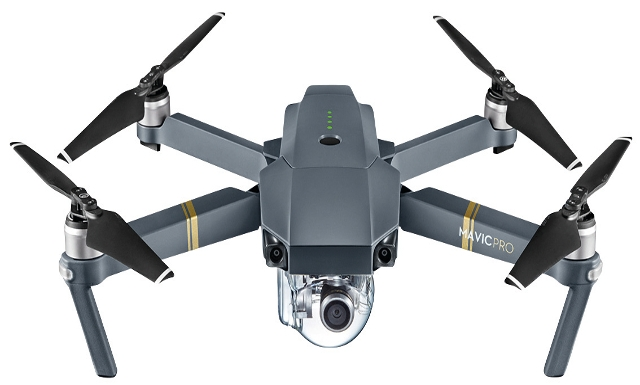
\includegraphics[width=.8\textwidth]{drone}
	\caption{DJI Mavic Pro \autocite{MavicProImage}}
	\label{drone}
\end{figure}

\newpage
\section{Voorbereiding van de software}

Na het klaar zetten van de drone, neemt de piloot de afstandsbediening en tablet bij zich en opent hij de reeds geïnstalleerde app Litchi. Nadat de app geopend is, navigeert hij naar de "Waypoint" modus waarin hij, manueel of bij voorkeur aan de hand van een template omdat dat sneller is, de verschillende navigatiepunten instelt (figuur \ref{waypoint}). Indien men een goed idee heeft van waar de drenkeling zich bevindt, kan men deze waypoints aanpassen zodat de drone meteen in de juiste richting vliegt. Een alternatief zou kunnen zijn om in alsmaar verder uitdeinende concentrische cirkels rond het schip te circuleren met de drone. Wanneer het pad ingesteld is, drukt men op de "play" toets waarna de drone automatisch dit pad zal volgen. In onze test wordt geopteerd voor een eenvoudige lus vanwege plaatsgebrek maar dit zal in het midden van de oceaan uiteraard niet het geval zijn. 

\begin{figure}[h]
	\centering
	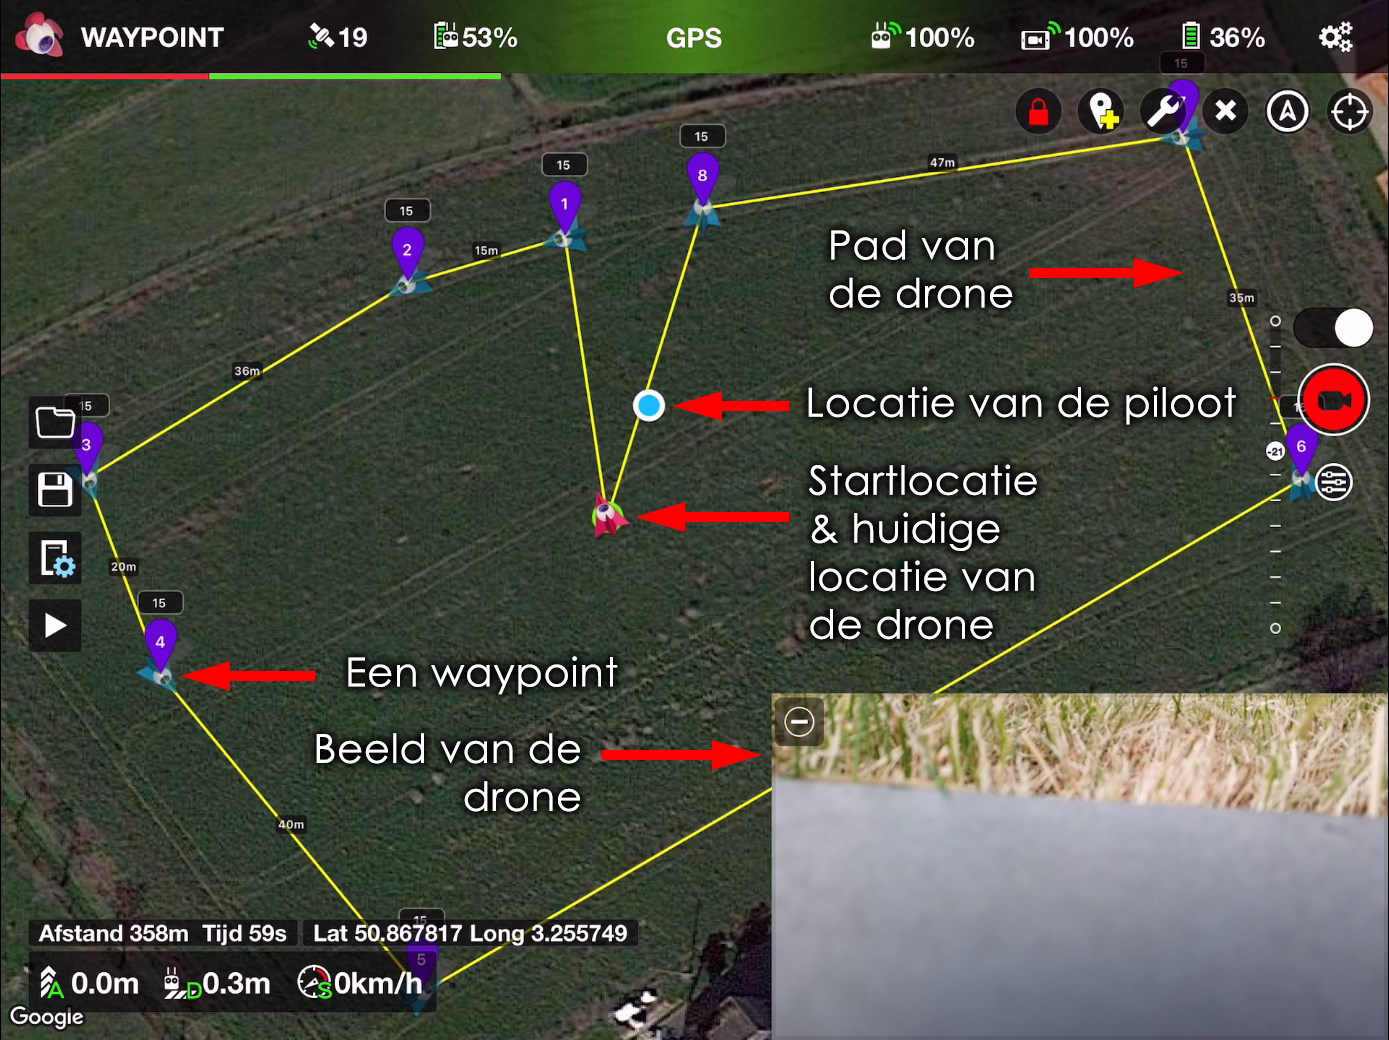
\includegraphics[width=.8\textwidth]{WAYPOINT}
	\caption{Een kaart van de locatie met de waypoints erop aangeduid}
	\label{waypoint}
\end{figure}


\section{Tijdens de vlucht}

De drone is nu vertrokken en volgt autonoom het ingestelde pad dankzij de Litchi app. Hoewel het detecteren van een drenkeling via de SDK (gemaakt en ter beschikking gesteld door DJI) wel geautomatiseerd zou kunnen worden, gaan wij gedurende de test op het zicht kijken wanneer de drenkeling op het scherm in beeld komt. In onze test is dit met een gewone camera wat op zich niet altijd de optimale oplossing is in donkere omstandigheden of in klaarlichte dag maar als we gebruik zouden maken van infra-rood en/of warmte camera's, zoals eerder besproken werd in hoofdstuk 2 en 3, dan zou het verschil tussen de drenkeling en de omgeving (oceaan) duidelijk genoeg zijn zodat dit geen probleem meer vormt.

\section{Gevonden!}

We hebben de drenkeling gevonden zoals je kan zien op figuur \ref{far}! Op dit moment moet de verantwoordelijke, de besturing van de drone even overnemen om hem correct te positioneren (figuur \ref{close}) waarna hij de "Active Tracking" functie kan activeren (figuur \ref{funcswitch}). Het exact positioneren van de drone zou opnieuw geautomatiseerd kunnen worden maar dit doen we in onze test niet. De "Active Tracking" functie is in staat om een object, dat aangeduid werd door de gebruiker, te volgen en in het midden van het beeld te houden (figuur \ref{activetrack}). Dan moet de crew van het schip slechts de coördinaten, die ze op het scherm waarop de app draait kunnen aflezen, door te geven aan de reddingsdiensten zodat zij een exacte locatie hebben om naartoe te navigeren. Van zodra de reddingsdiensten ter plaatse zijn, is het de taak van de bestuurder van de drone om deze op tijd weg te navigeren van de drenkeling zodat de reddingsoperatie niet bemoeilijkt wordt.

\newpage

\begin{figure}[h]
	\centering
	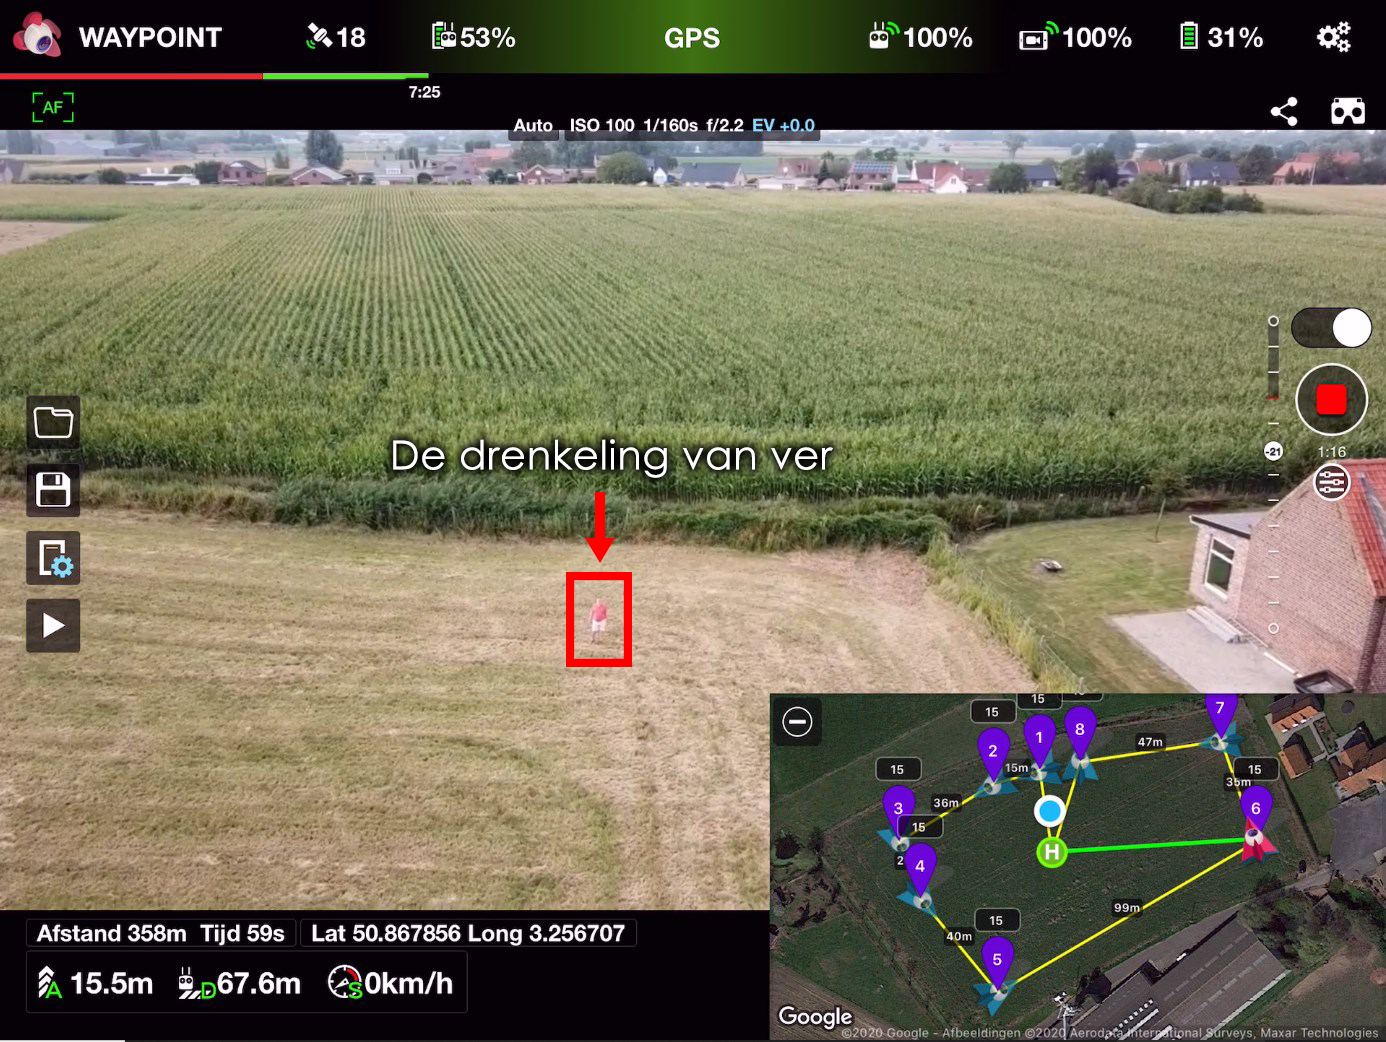
\includegraphics[width=.7\textwidth]{DRENKELING_VER}
	\caption{De drenkeling wanneer hij van ver gezien wordt.}
	\label{far}
\end{figure}
\begin{figure}[h]
	\centering
	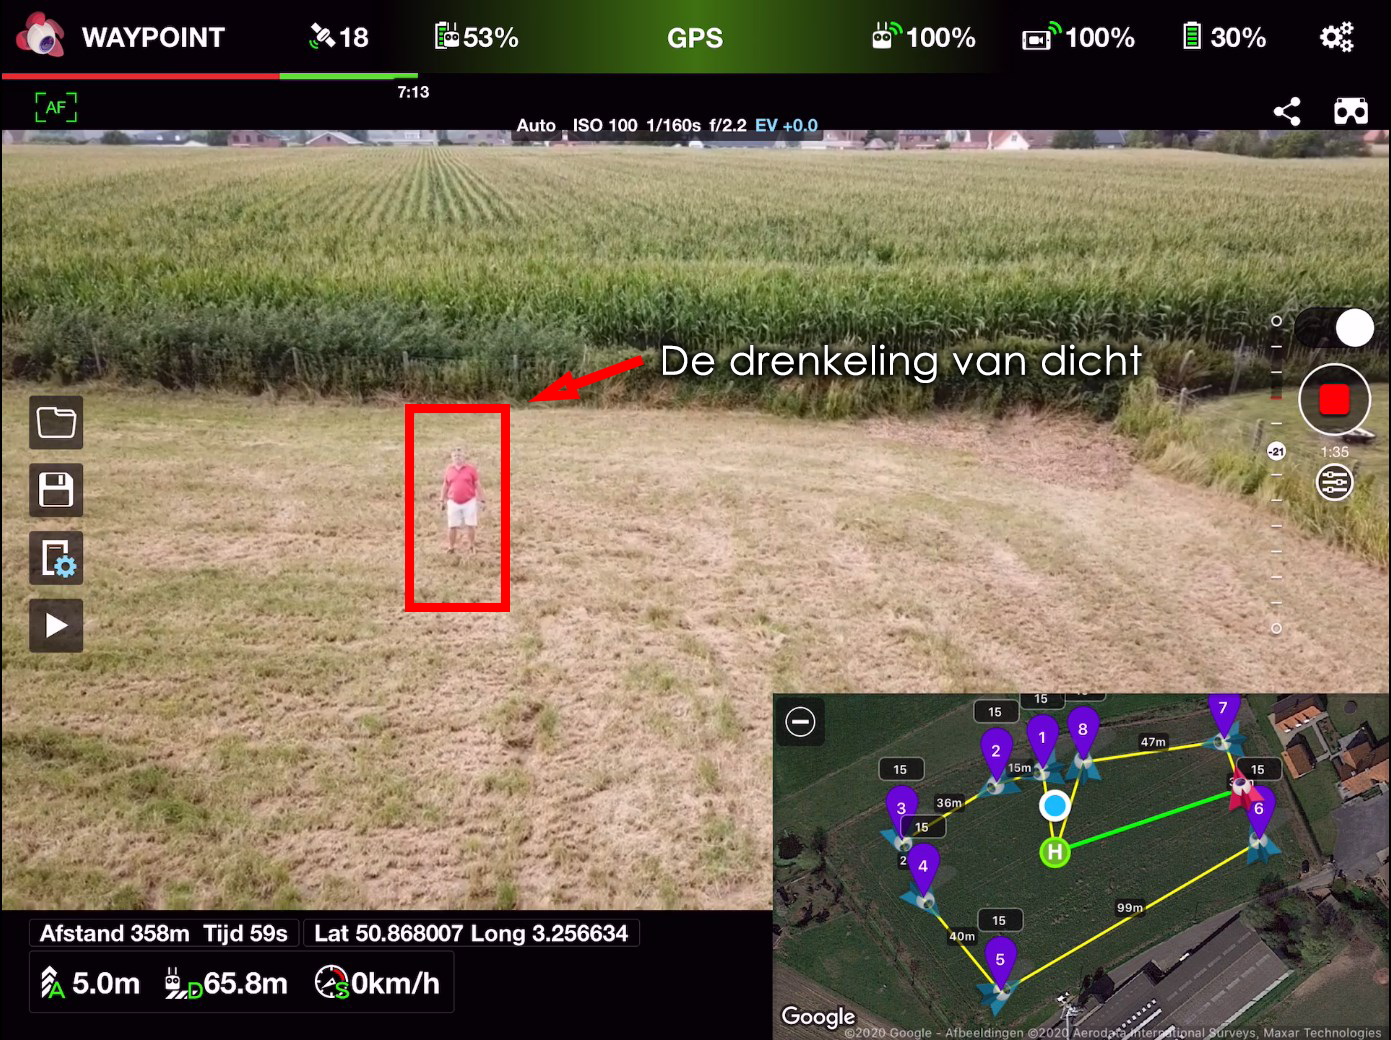
\includegraphics[width=.7\textwidth]{DRENKELING_DICHT}
	\caption{De drenkeling nadat de drone correct gepositioneerd is.}
	\label{close}
\end{figure}

\newpage

\begin{figure}[h]
	\centering
	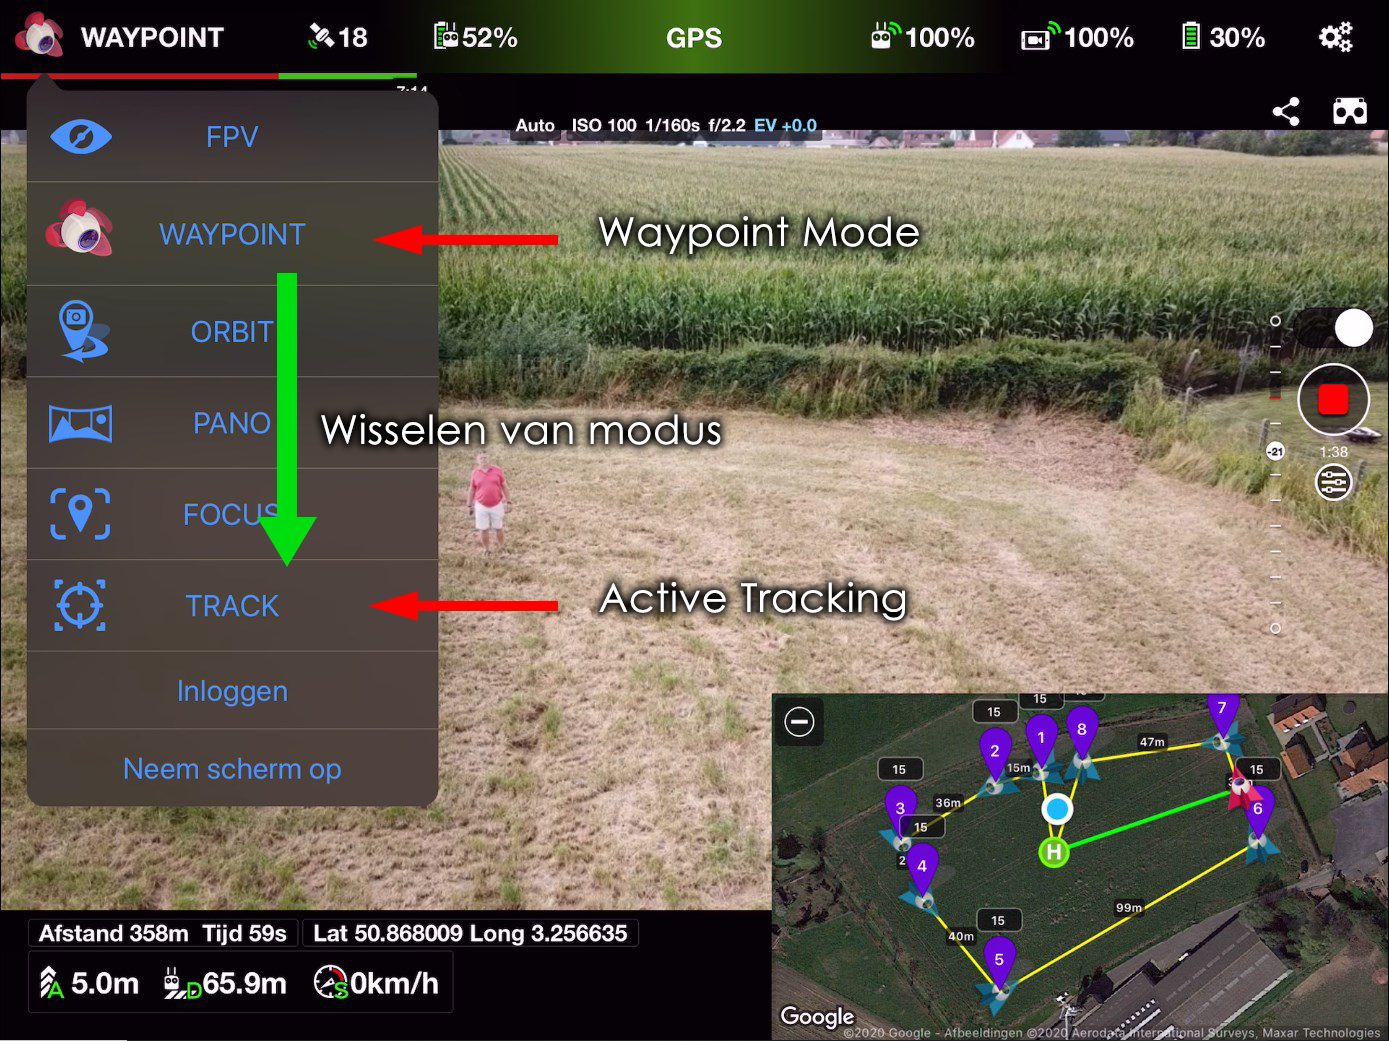
\includegraphics[width=.7\textwidth]{FUNCTIONALITEITEN}
	\caption{Het functionaliteitenmenu van de Litchi app. Bevat o.a. waypoint en tracking}
	\label{funcswitch}
\end{figure}
\begin{figure}[h]
	\centering
	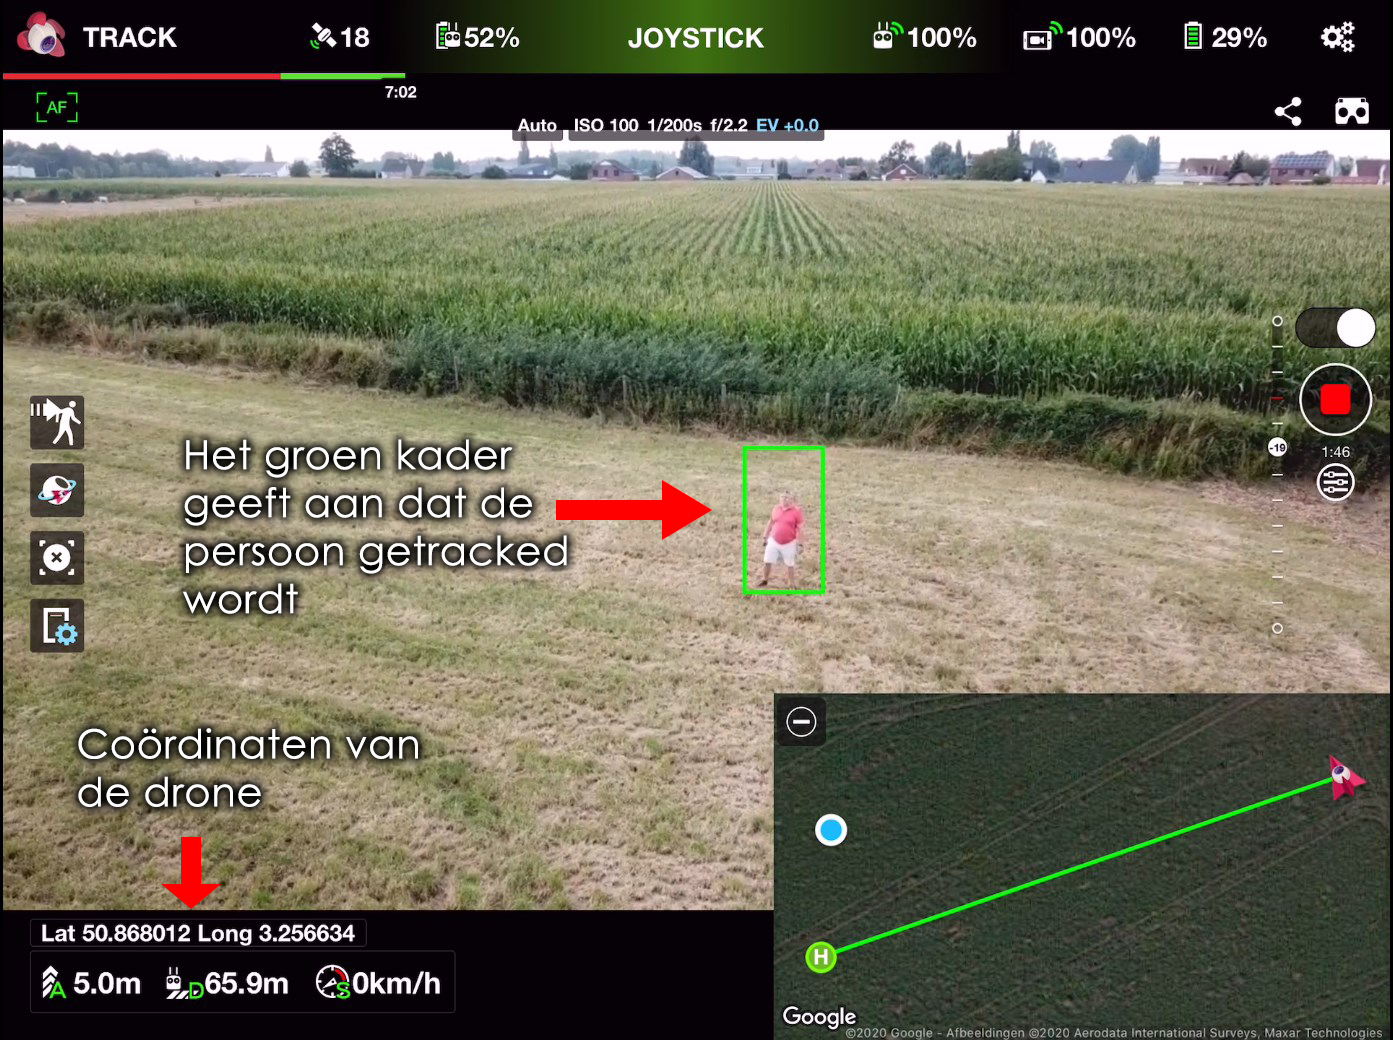
\includegraphics[width=.7\textwidth]{ACTIVE_TRACKING}
	\caption{De app tijdens active tracking}
	\label{activetrack}
\end{figure}

\newpage

\section{Bevindingen}

Tijdens het uitvoeren van ons scenario hebben we het volgende vastgesteld:

\begin{itemize}
	\item De ''Waypoint'' functionaliteit van de Litchi app werkte heel erg goed. De drone was in staat om het vooraf ingestelde pad zonder problemen te volgen.
	\item De ''Active Tracking'' functionaliteit van de Litchi app werkte niet zo goed. Het verloor zijn ''zicht'' op de drenkeling na enkele seconden waardoor we het kader rond de ''drenkeling'' ook dikwijls moesten hertekenen.
\end{itemize}

Wil dit dan zeggen dat ''Active Tracking'' een technologie is die nog niet op punt staat? Nee, het werkt namelijk perfect op de app die door DJI zelf ontwikkeld is. Zelfs op een hoogte van 10-15 meter, wanneer het lichaam van een persoon veel kleiner is, kon de drone onze drenkeling nog steeds volgen en in beeld houden. Het is dus vooral de Litchi Active Tracking die nog geoptimaliseerd moet worden. Ondanks het feit dat de technologie nog niet helemaal op punt staat, zijn er duidelijk mogelijkheden genoeg die voldoen aan de vereisten van onze toepassing.

% Voeg hier je eigen hoofdstukken toe die de ``corpus'' van je bachelorproef
% vormen. De structuur en titels hangen af van je eigen onderzoek. Je kan bv.
% elke fase in je onderzoek in een apart hoofdstuk bespreken.

%\input{...}
%\input{...}
%...

%%=============================================================================
%% Conclusie
%%=============================================================================

\chapter{Conclusie}
\label{ch:conclusie}

% TODO: Trek een duidelijke conclusie, in de vorm van een antwoord op de
% onderzoeksvra(a)g(en). Wat was jouw bijdrage aan het onderzoeksdomein en
% hoe biedt dit meerwaarde aan het vakgebied/doelgroep? 
% Reflecteer kritisch over het resultaat. In Engelse teksten wordt deze sectie
% ``Discussion'' genoemd. Had je deze uitkomst verwacht? Zijn er zaken die nog
% niet duidelijk zijn?
% Heeft het onderzoek geleid tot nieuwe vragen die uitnodigen tot verder 
%onderzoek?

We hebben de hardware, de software en de implementatie van een on-board drone besproken en kunnen besluiten dat dit de beste manier van aanpak is. 

Van cruciaal belang is het feit dat op Europees en/of globaal vlak een éénduidige wetgeving tot stand komt zodat dit concept kan geïmplementeerd worden. 

Eens dat er is, kunnen we de duurdere drone gebruiken die standaard uitgerust is met een warmtecamera en een infrarood camera alsook een systeem dat ons in staat stelt om zaken te transporteren. 

Vervolgens zullen we een groot volume voorbeeldfoto's moeten maken om deze onder te verdelen tussen training- en testdataset. Pas daarna kunnen we het klassificatie-algoritme trainen en aan de hand van de testdataset, de accuraatheid gaan testen. Eens de accuraatheid van het algoritme op punt staat, kunnen we het algoritme in gebruik gaan nemen. 

Verder kunnen we de drone verder gaan uitrusten met een extra microfoon, luidspreker, een reddingsboei of module die de drone omvormt tot een reddingsband en het belangrijkste onderdeel, een lokalisatiezender zodat de locatie doorgegeven kan worden aan zowel de bemanning van het schip als de reddingsdiensten. 

Tot slot kunnen we nog het softwarepakket gaan maken dat de drone in staat stelt om de kustwacht, verantwoordelijk voor de wateren waarin het schip zich bevindt, te verwittigen van het incident alsook andere gegevens zoals de locatie van het incident door te geven. Ook zal het softwarepakket instaan voor de verdere communicatie tussen de crew van het schip en diezelfde kustwacht.

De stappen die men moet ondernemen in het geval van een man-over-boord situatie zijn de volgende:

De eerste stap is het lanceren van de drone zodat deze een signaal geeft aan de respectievelijke reddingsdiensten. Vervolgens wordt er gewacht op het contact met de reddingsdiensten. Deze hebben ondertussen de locatie reeds doorgegeven aan de reddingsoperatoren. Verder advies kan gegeven worden door de reddingsdiensten aan de crew. Tenslotte kan de drone, éénmaal de drenkeling gevonden is, de locatie doorgeven zodat de reddingsdiensten (of de crew indien de reddingsdiensten nog niet aangekomen zijn) kunnen overgaan tot de effectieve reddingsoperatie.

Na het uitvoeren van de proof-of-concept, kunnen we nu met zekerheid zeggen dat de technologieën, die op dit moment op de markt beschikbaar zijn, zeker volstaan om dit concept volledig uit te werken. Het is zelfs mogelijk om de drone alles op een volledig autonome manier te laten uitvoeren. Zeker met de duurdere drones die veel flexibeler geprogrammeerd kunnen worden dankzij de extra sensoren, betere vliegperformantie en andere optionele uitbreidingen moet dit concept zonder twijfel gerealiseerd kunnen worden. Het is echter wel zo dat dit een omvangrijk project zal zijn aangezien, zoals eerder al vermeld, er heel wat invalshoeken zijn waarmee rekening moet gehouden worden. Voor dergelijk project kunnen de kosten hoog oplopen en zal de tijd die dit in beslag kan nemen aanzienlijk zijn. Kosten noch moeite mogen echter gespaard blijven wanneer we het hebben over het redden van een mensenleven.

 



%%=============================================================================
%% Bijlagen
%%=============================================================================

\appendix
\renewcommand{\chaptername}{Appendix}

%%---------- Onderzoeksvoorstel -----------------------------------------------

\chapter{Onderzoeksvoorstel}

Het onderwerp van deze bachelorproef is gebaseerd op een onderzoeksvoorstel dat vooraf werd beoordeeld door de promotor. Dit voorstel is opgenomen in deze bijlage.

% Verwijzing naar het bestand met de inhoud van het onderzoeksvoorstel
%---------- Inleiding ---------------------------------------------------------

\section{Introductie} % The \section*{} command stops section numbering
\label{sec:introductie}

\textbf{Het probleem}\\
Jaarlijks sterven gemiddeld 320.000 mensen door verdrinken. Het grootste deel in overspoelingsrampen maar ook vissers lopen een verhoogd risico. Stel dat een visser per ongeluk in de oceaan valt tijdens het doorvaren van een omgeving met sterk beperkt zicht, dan is het cruciaal om de drenkeling zo spoedig mogelijk op te sporen. Hoe langer de drenkeling vermist blijft, hoe verder hij/zij afgevoerd kan worden door de stromingen van de oceaan en dus hoe kleiner de kans dat de drenkeling terug gevonden wordt voordat onderkoeling of vermoeidheid optreedt. Eens vermoeidheid of onderkoeling optreedt is de kans op overlijden des te groter.\\\\
\textbf{De oplossing}\\
De dag van vandaag zijn er al heel wat optische technologieën beschikbaar die, in combinatie met de juiste software, in staat zijn om mensen te detecteren. Er zijn ook drones die door relatief barre weersomstandigheden kunnen navigeren zonder veel problemen en nog belangrijker, aan hoge snelheid. Daarom zou de combinatie van deze twee technologieën, een zeer effectieve manier kunnen zijn om drenkelingen snel op te sporen.\\\\
\textbf{Doelstelling \& onderzoeksvragen}\\
Het doel van deze bachelorproef is het vinden van de beste optische technologie(ën) voor het opsporen van drenkelingen bij bepaalde weersomstandigheden.\\\\
\underline{onderzoeksvragen:}\\
Is er een optische technologie superieur ten opzichte van alle andere technologieën?\\ Zoniet, welke technologie is het beste voor welke omstandigheden?

%---------- Stand van zaken ---------------------------------------------------

\section{State-of-the-art}
\label{sec:state-of-the-art}

Drones worden reeds gebruikt voor het assisteren van reddingsoperaties in verscheidene andere omgevingen zoals bijvoorbeeld rampgebieden (aardbevingen, tornado's, overstromingen, ...)\autocite{DronesAndDisaster}, bergketens of gebieden met heuvelachtige eigenschappen \autocite{Mountains} en oorlogsgebieden. Het is dus zonder twijfel mogelijk om drones in barre weersomstandigheden in te zetten.\\\\
Er is reeds onderzoek gedaan naar het detecteren van personen aan de hand van infra-rood camera's zoals beschreven in \autocite{IR} Gezien er weinig andere organismen met eenzelfde grote infra-roodsignatuur zullen zijn, is het niet onwaarschijnlijk dat dit een goede oplossing zou kunnen zijn voor ons probleem.\\\\
Voor het gebruiken van warmtecamera's is er ook al heel wat onderzoek gedaan. \autocite{Heat} beschrijft een onderzoek waarbij men personen of objecten detecteert aan de hand van een klassificatiealgoritme (onderdeel van machineleren) op zee en ze daarna ook te volgen.\\\\ Ten slotte is er nog nachtzicht cameras. Dit is nog een andere soort camera die ook organismen met een lichaamswarmte via kleuren aanduidt. Ook bij dit type camera is er reeds onderzoek uitgevoerd voor het detecteren van mensen. In dit onderzoek werden 2 soorten algoritmen onderzocht met als doel, het vinden van het algoritme met de beste nauwkeurigheid. \autocite{Night}\\\\
Voor het herkennen van mensen op basis van verkregen beelden kan, zoals hierboven vermeld werd, een klassificatiealgoritme gebruikt worden. Dit is een algoritme die tot toebehoort machineleren. Zo kan men tegenwoordig reeds aan veel gecompliceerdere objectherkenning doen dan wij in ons geval nodig zullen hebben. Meer over klassificatiealgotirmen worden besproken in \autocite{Classification}.

% Voor literatuurverwijzingen zijn er twee belangrijke commando's:
% \autocite{KEY} => (Auteur, jaartal) Gebruik dit als de naam van de auteur
%   geen onderdeel is van de zin.
% \textcite{KEY} => Auteur (jaartal)  Gebruik dit als de auteursnaam wel een
%   functie heeft in de zin (bv. ``Uit onderzoek door Doll & Hill (1954) bleek
%   ...'')


%---------- Methodologie ------------------------------------------------------
\section{Methodologie}
\label{sec:methodologie}

Tijdens dit onderzoek zal er aan de hand van verscheidene soorten camera's en een klassificatiealgoritme nagegaan worden welke camera's het beste presteren bij welke weersomstandigheden. We zullen bij verschillende weersomstandigheden en op verschillende afstanden nagaan of een persoon gedetecteerd wordt. Zoals eerder vermeld gaan we gebruik maken van klassificatiealgoritmes die de pixels met een persoon in een aparte klasse klassificeert om zo de drenkeling te vinden. Dit algoritme zal wel eerst getrained moeten worden vooraleer aan herkenning gedaan kan worden.

%---------- Verwachte resultaten ----------------------------------------------
\section{Verwachte resultaten}
\label{sec:verwachte_resultaten}

Als resultaat verwachten we dat elke camera zijn sterktes en zwaktes zal hebben. Bij de ene set weersomstandigheden zal camera A misschien superieur zijn terwijl bij andere weersomstandigheden camera B dan weer superieur zal zijn. 

%---------- Verwachte conclusies ----------------------------------------------
\section{Verwachte conclusies}
\label{sec:verwachte_conclusies}

Ik verwacht dat camera's zoals warmtecamera's en infraroodcamera's met de hoogste efficientie te werk zullen gaan. Een gewone camera maakt te weinig onderscheid tussen organismen en de omgeving. Daarboven denk ik dat warmtecamera's nog efficienter zullen zijn dan infra-roodcamera's. Indien mensen in een reddingsboot erin slagen om een noodfakkel aan te steken bij het passeren van een drone, dan zullen ze zeker opgemerkt worden door een warmtecamera. 



%%---------- Andere bijlagen --------------------------------------------------
% TODO: Voeg hier eventuele andere bijlagen toe
%\input{...}

%%---------- Referentielijst --------------------------------------------------

\printbibliography[heading=bibintoc]

\end{document}
